



To optimize the software energy consumption, a reproducible setup environment requires to be designed.

This chapter will be dedicated to provide a set of guidelines to provide a \em{reproducible, accurate} and \em{representative} tests. Each aspect will be detailed in the sections below.


\section{Threats and Challenges}
A successful benchmark has three criterions to fullfil.
First, it has to be \emph{reproducible} for others to replicate.
Second, the results should be \emph{accurate}, which means each time we rerun the benchmark we are expecting the same results.
Finally, it should \emph{represent} the real world.
In other words, the conclusions brought from the experiment should be valid outside the experimentation as well.
In my case, the real world is the production environment.
Therefore, our experiments should reflect what is happening in the production environments.
In this section, I will deeper dig in each aspect, present what has been done by others and my contributions, and finally I will propose some perspectives, to improve such experiments.

%%%%%%%%% preliminary taughts and section structure 
% The need of reproducibility in our field - software optimization based on empirical studies -

% The importance of Virtualisation for reproducibility \cite{howe_virtual_2012}
% some of the most important parts are
% - fewer constraints on research methods
% - on-demand backups
% - virtual Machines as Publications
% - more Variables captured

\subsection{Reproducibility}
One of the most difficult challenges faced by researchers is the reproducibility of their benchmarks.
Actually, many results fail to be reproduced,\footnote{Trouble at the lab, The Economist, 19 October 2013;  www.economist.com/news/briefing/ 21588057-scientists-think-science-self-correcting- alarming-degree-it-not-trouble.} which led to a \emph{replication crisis}.
As this crisis hit most of the empirical studies, most of the reviews now includes reproducibility as one of the minimal standard for judging scientific merit.\cite{peng2011reproducible}
One of the criterions supporting reproducibility is the publication of the dataset and the algorithms run on the raw data to conclude the results.
There is even some disagreement about what the terms "reproducibility" or "replicability" by themselves mean \cite{goodman2016does}.
According to \cite{echtler2018open}, \emph{replicability} extends \emph{reproducibility} with the ability to collect a new raw dataset comparable to the original one by re-executing the experiment under similar condition, instead of just the ability to get the same results by running the statistical analyses on the original data set.

In the area covered by this PhD thesis, reproducibility might be achieved by ensuring the same execution settings of physical nodes, virtual machines, clusters or cloud environments.
However, when it comes to measuring the energy consumption of a system, applying acknowledged guidelines and carefully repeating the same benchmark can nonetheless lead to different energy footprints not only among homogeneous nodes, but even within a single node.

One major problem that hinders the reproducibility of the empirical benchmarks is the interaction with the external environment, either as concurrency or dependencies.
Therefore, researchers cannot observe the same results, unless they duplicate the same environment.


\subsection{Accuracy}
According to Oxford, \emph{accuracy} means \href{https://www.lexico.com/definition/accuracy}{"technical The degree to which the result of a measurement, calculation, or specification conforms to the correct value or a standard"}.
In ny case, this means the ability to run the benchmark multiple times with a low variation.

Recently, the research community has been investigating typical "crimes" in systems benchmarking and established guidelines for conducting robust and reproducible evaluations~\cite{DBLP:journals/corr/abs-1801-02381}.

In theory, using identical CPU, same memory configuration, similar storage and networking capabilities, should increase the accuracy of physical measurements.
Unfortunately, this is not possible when it comes to measuring the energy consumption of a system.
Applying the benchmarking guidelines and repeating the same experiment with in the same configuration are not sufficient to reproduce the the same energy measurements, not only between identical machines, but even within the same machine.
This difference---also called \emph{energy variation} (EV)---has become a serious threat to the accuracy of experimental evaluations.

%TODO:  rephrase this figure, maybe change it a little bit 
Figure~\ref{fig:motivation} illustrates this variation problem as a violin plot of $20$ executions of the benchmark \emph{Conjugate Gradient} (\textsf{CG}) taken from the \emph{NAS Parallel Benchmarks} (NBP) suite~\cite{Bailey:1991:NPB:125826.125925}, on $4$ nodes of an homogeneous cluster (the cluster \textsf{Dahu} described in Table~\ref{table:g5k}) at 50\,\% workload.
We can observe a large variation of the energy consumption, not only among homogeneous nodes, but also at the scale of a single node, reaching up to $25\,\%$ in this example.

\begin{figure}%[!htb]
    \center{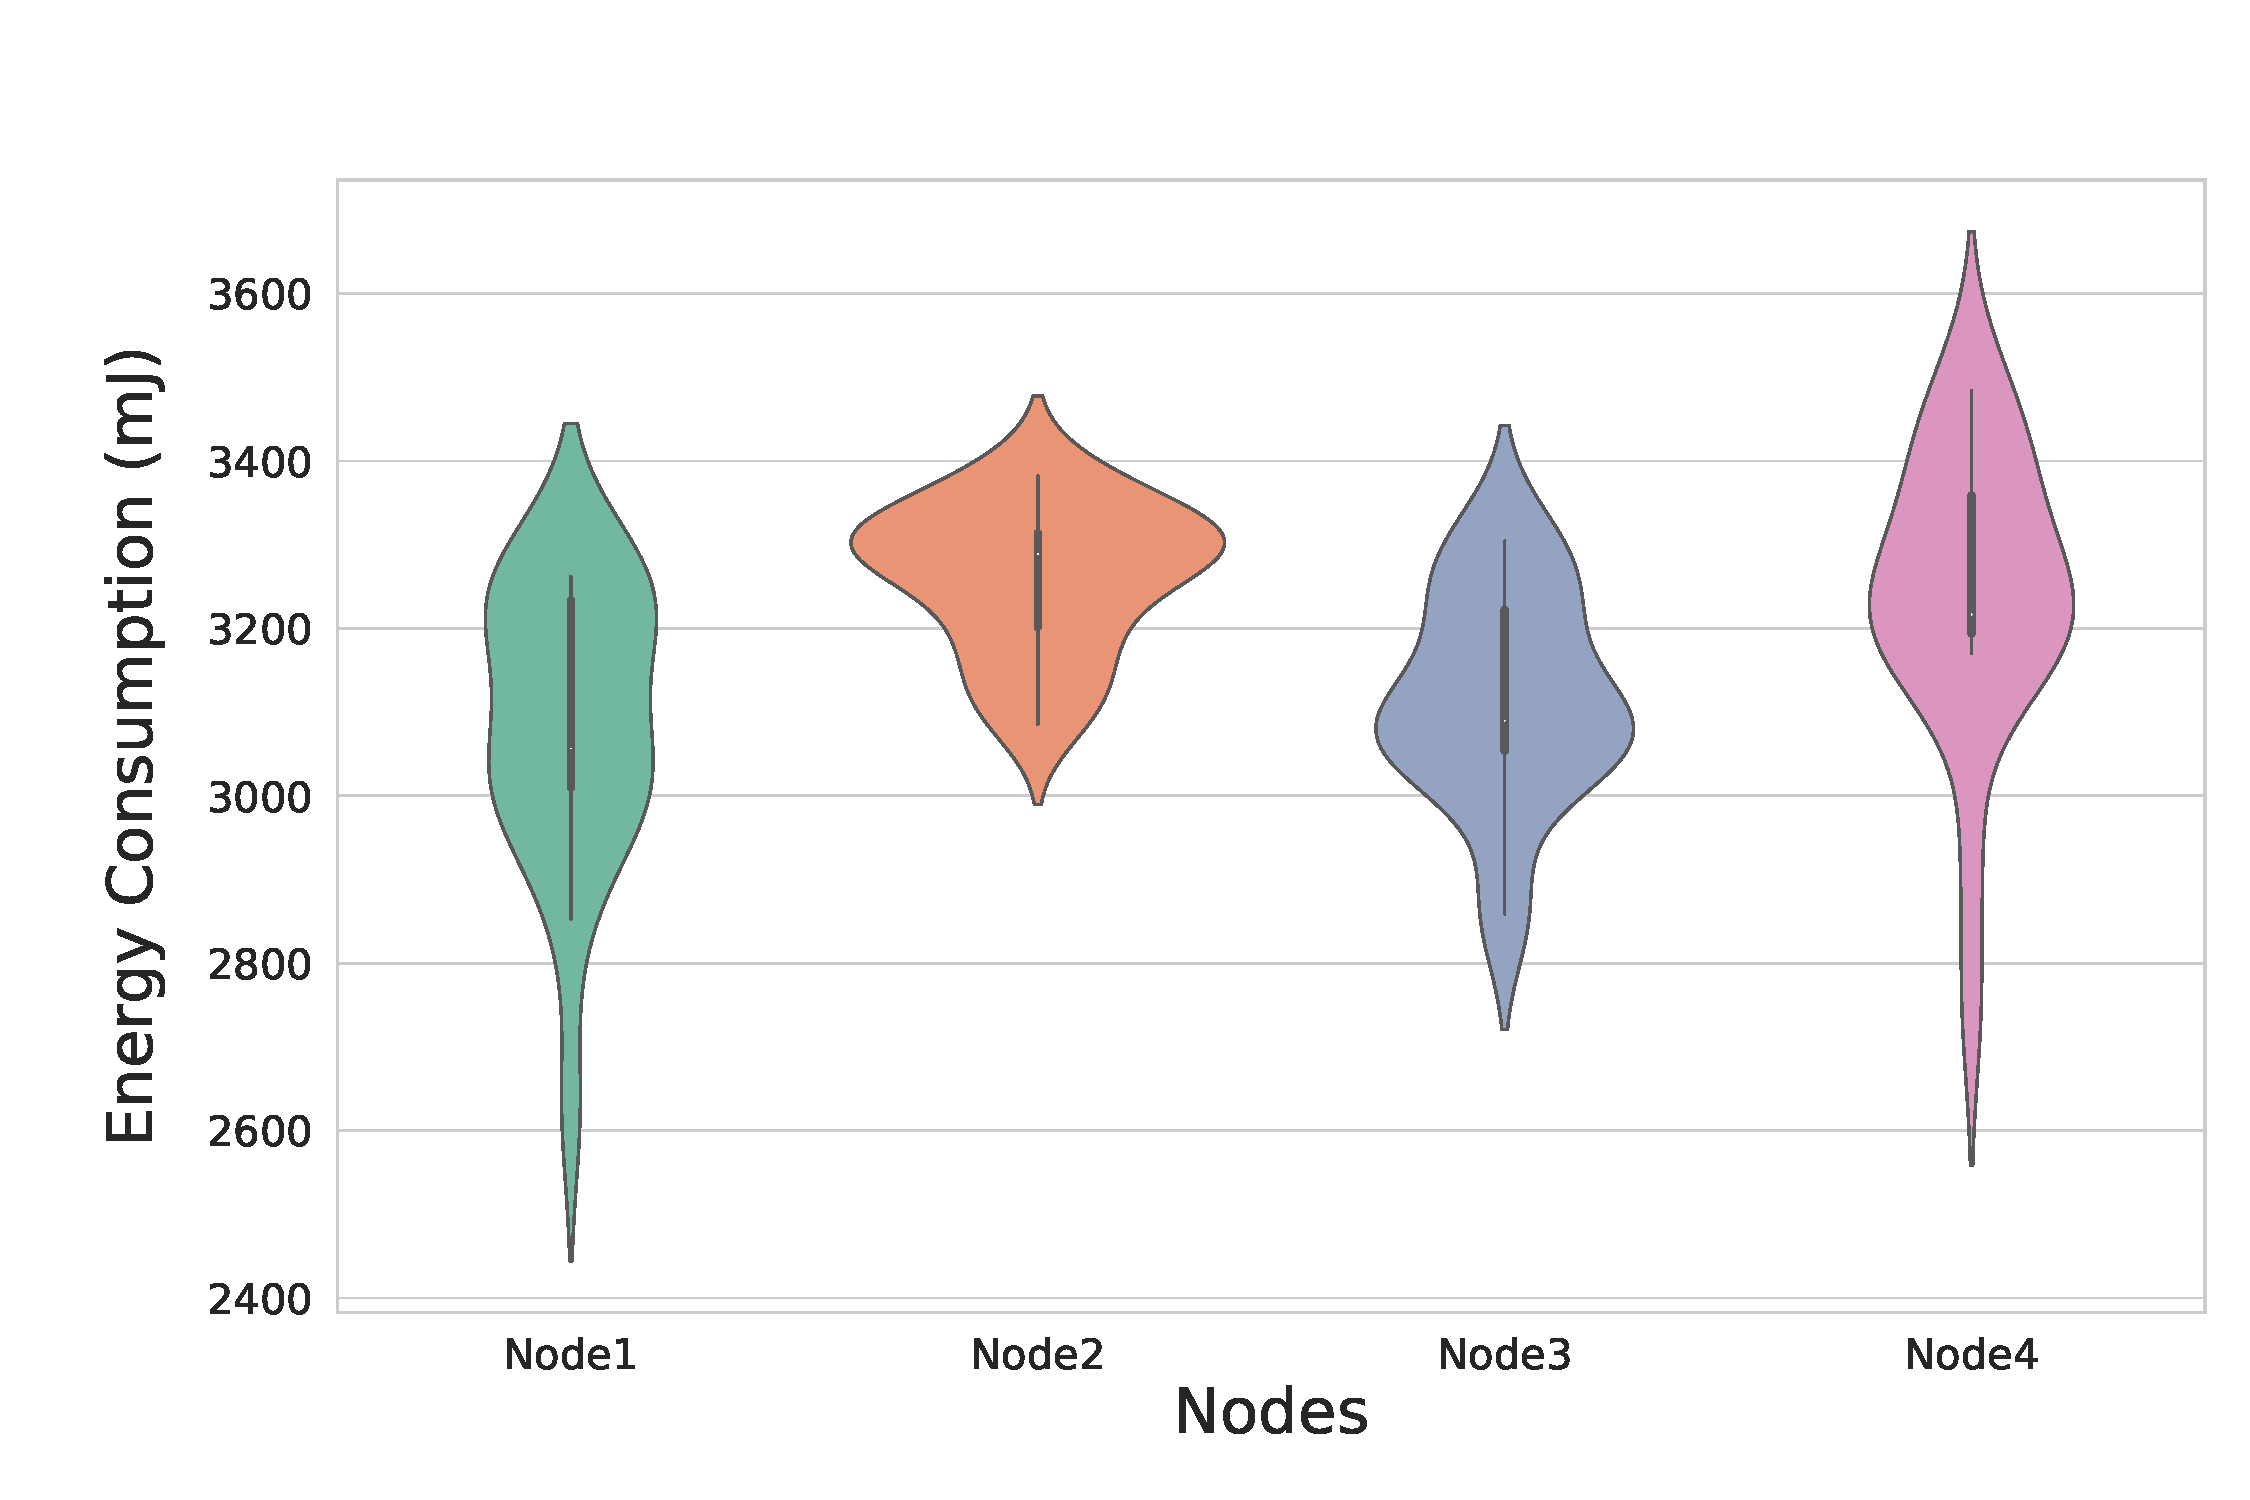
\includegraphics[width=.9\linewidth]{imgs/motivation}}
    \caption{CPU energy variation for the benchmark \textsf{CG}}\label{fig:motivation}
\end{figure}

Some researchers started investigating the hardware impact of the energy variation of power consumption.
As an example, one can cite~\cite{borkar_designing_2005,tschanz_adaptive_2002} who reported that the main cause of the variation of the power consumption between different machines is due to the \textbf{CMOS} manufacturing process of transistors in a chip.
\cite{heinrich_predicting} described this variation as a set of parameters, such as CPU Frequency and the thermal effect.


\subsection{Representativeness}
As obvious as it seems, the reason of executing benchmarks is to validate ideas so we can use them in the real life.
However, this is means that those benchmarks have to represent reality somehow.
Basically, when we aim to benchmark something, we create a mock up version of the situation that we want it to work.
% But, how can we assure that the benchmark is representative? honestly i don't know. and we can't generalize this. but there are some works that have been done for this.
First, we can talk about the benchmarking and their selection, then we will talk about the stress benchmark for some applications, and finally we will bring this representativeness in our case and how can we get closer to the energy consumption behavior of a software between the benchmark environnement and the production one.

As Stephen M. Blackburn~\emph{et~al.} cited in their paper "evaluate collaboratory"~\cite{stephen_evaluate_2012}, one of the major pitfalls of the measurement contexts is the inconsistency, which can be translated here by the fact that the production context is not the same as the benchmarking one.

Another difficult part for practitioners is to generalize the claims they reached beyond the lab conditions.
Are they appropriate?
Are they consistent and are they reproducible?
To answer those questions, the community agreed on some wellknown benchmarks to represent a specific concern of the production world.
One can site as an example the Dacapo and Renaissance benchmark suites for Java applications, or the CLBG benchmark suite for comparing programming languages.
Although they do not cover all the cases, the community agrees on their relevance and representativeness.

In addition to those benchmarks, a new category of benchmarking technique emerged to simulate the worst case of the production environments, inlcuding performance tests, which are benchmarks meant to evaluate the behavior of a software under stress situations.
We can cite as an example the Gatling for web application and stress-ng for hardwares.%ROMAIN: Add citations.
%% YEP I KNOW, THIS IS JUST FOR ME TO READ IT LATER AND GIVE A BETTER CONTEXT



%  TODO: add the environement part,
%  TODO: add perspective 

\section{Experimental Guidelines}\label{sec:guidelines}
To summarize our experiments, we provide some experimental guidelines in Table~\ref{table:guidelines}, based on the multiple experiments and analysis we did.
These guidelines constitute a set of minimal requirements or best practices, depending on the workload and the criticality of the energy measurement precision.
It therefore intends to help practitioners in taming the energy variation on the selected CPU, and conduct the experiments with the least variations.

\begin{table}[h!]
    \centering
    \caption{Experimental Guidelines for Energy Variations}
    \small
    \begin{tabular}{|p{4.7cm}|c|c|}
        \hline
        \textbf{Guideline}                                                                                                                                                & \textbf{Load} & \textbf{Gain}     \\
        \hline
        \hline
        Use a low TDP CPU                                                                                                                                                 & Low \& medium & Up to $3\times$   \\
        \hline
        Disable the CPU C-states                                                                                                                                          & Low           & Up to $6\times$   \\
        \hline
        Use the least of sockets in a case of multiple CPU                                                                                                                & Medium        & Up to $30\times$  \\
        \hline
        Avoid the usage of hyper-threading whenever possible                                                                                                              & Medium        & Up to $5\times$   \\
        \hline
        Avoid rebooting the machine between tests                                                                                                                         & High          & Up to $1.5\times$ \\
        \hline
        Do not relate to the machine idle variation to isolate a test EC, the CPU/OS changes its behavior when a test is running and can exhibit less variation than idle & Any           & ---               \\
        \hline
        Rather focus the optimization efforts on the system under test than the OS                                                                                        & Any           & ---               \\
        \hline
        Execute all the similar and comparable experiments on a same machine. Identical machines can exhibit many differences regarding their energy behavior             & Any           & Up to $1.3\times$ \\
        \hline
    \end{tabular}
    \label{table:guidelines}
\end{table}

Table~\ref{table:guidelines} gives a proper understanding of known factors, like the C-states and its variation reduction at low workloads.
However, it also lists some new factors that we identified along the analysis we conducted in Section, such as the results related to the OS or the reboot mode.
Some of the guidelines are more useful/efficient for specific workloads, as showed in our experiments.
Thus, qualifying the workload before conducting the experiments can help in choosing the proper guidelines to apply.
Other studied factors are not been mentioned in the guidelines, like the Turbo~Boost or the Speculative execution, due to the small effect that has been observed in our study.

In order to validate the accuracy of our guidelines among a varied set of benchmarks on one hand, and their effect on the variation between identical machines on the other hand, we ran seven experiments with benchmarks and real applications on a set of four identical nodes from the cluster \textsf{Dahu}, before (\textsf{normal} mode where everything is left to default and to the charge of the OS) and after (\textsf{optimized}) applying our guidelines.
Half of these experiments has been performed at a 50\,\% workload and the other half on single process jobs.
The choice of these two workloads is related to the optimization guidelines that are mainly effective at low and medium workloads.
We note that we used the cluster \textsf{Dahu} over \textsf{Ecotype} to highlight the guidelines effect on the nodes where the variation is susceptible to be higher.

\begin{figure*}%[!htb]
    \center{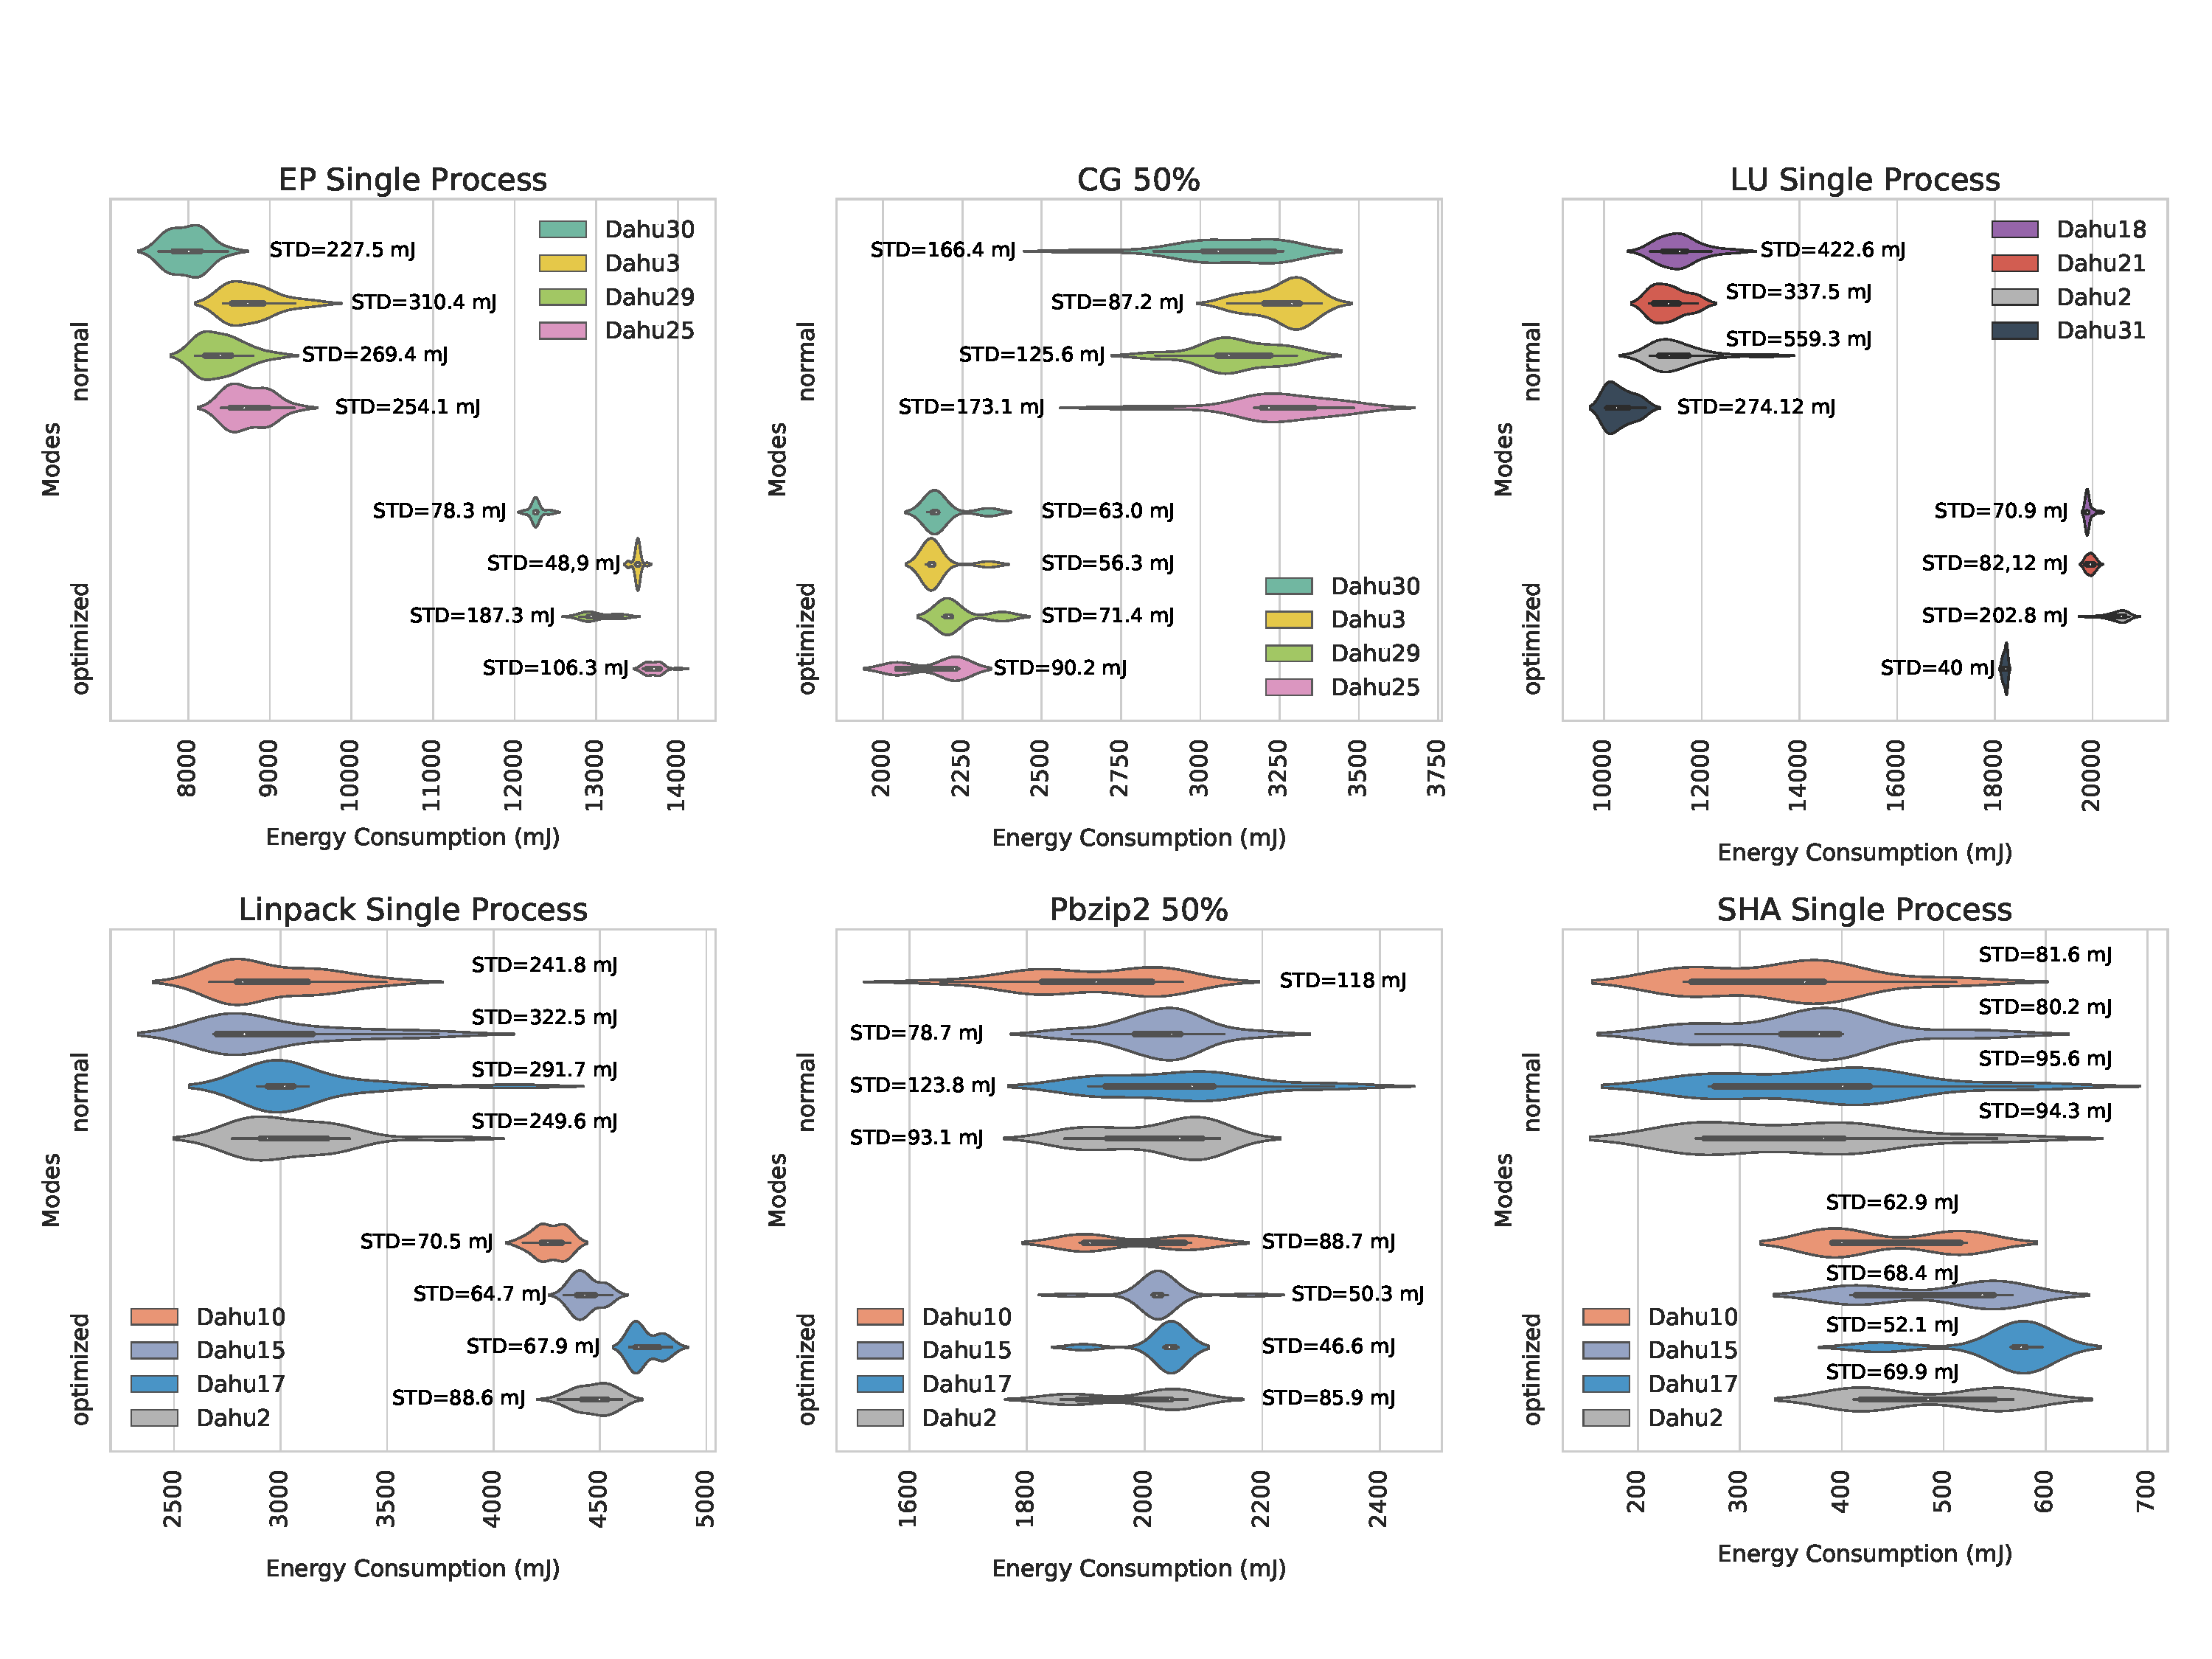
\includegraphics[width=\linewidth]{imgs/all}}
    \caption{Energy variation comparison with/without applying our guidelines}\label{fig:optimized}
\end{figure*}

\begin{figure}%[!htb]
    \center{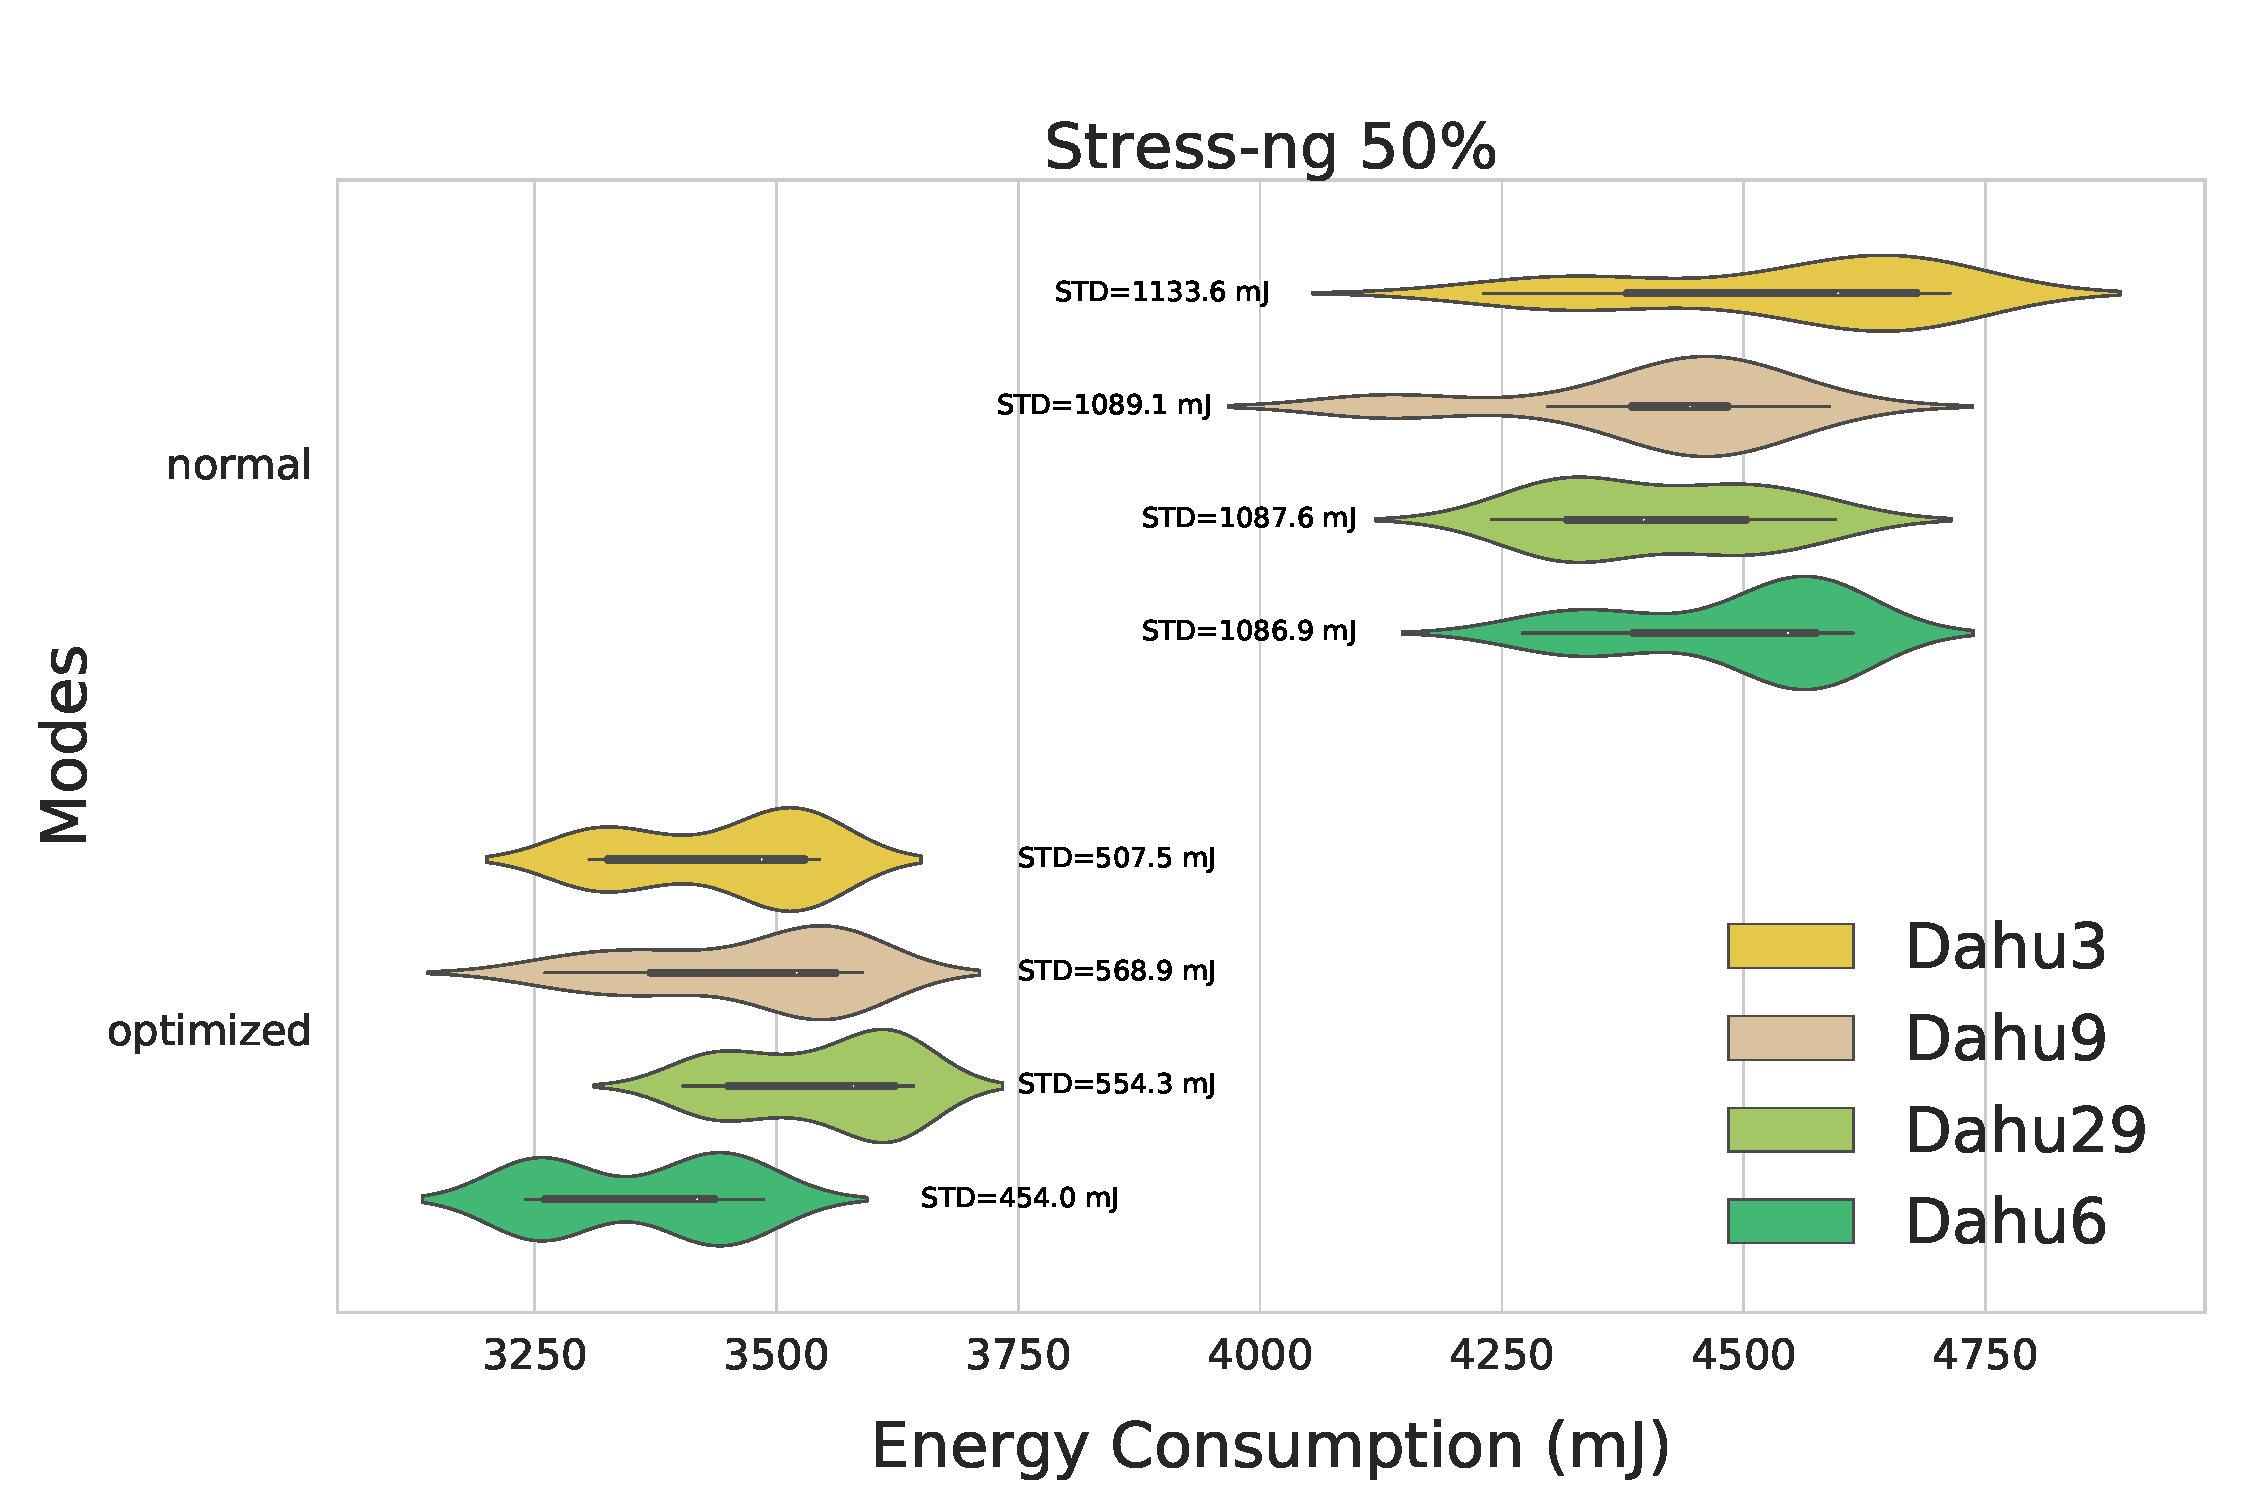
\includegraphics[width=.9\linewidth]{imgs/stressng}}
    \caption{Energy variation comparison with/without applying our guidelines for \textsc{Stress-NG}}\label{fig:stress}
\end{figure}

Figure~\ref{fig:optimized} and~\ref{fig:stress} highlight the improvement brought by the adoption of our guidelines.
They demonstrate the intra-node STD reduction at low and medium workloads for all the benchmarks used at different levels.
Concretely, for low workloads, the energy variation is 2--6 times lower after applying the optimization guidelines for the benchmarks \textsf{LU} and \textsf{EP}, as well as \textsc{Linpack}, while it is 1.2--1.8 times better for \texttt{Sha256}.
For this workload, the overall energy consumption after optimization can be up to 80\,\% higher due to disabling the C-states to keep all the unused cores at a high power consumption state ($Mean_{LU-normal-Dahu2}=11,500 mJ$, $Mean_{LU-optimized-Dahu2}=20,508 mJ$).
For medium workloads, the STD, and thus variation, is up to 100\,\% better for the benchmark \textsf{CG}, 20--150\,\% better for the \texttt{pbzip2} application and up to 100\% for \textsc{Stress-NG}.
We note that the optimized version consumes less energy thanks to an appropriate core pinning method.

Figures~\ref{fig:optimized} and~\ref{fig:stress} also highlight that applying the guidelines does not reduce the inter-nodes variation in all the cases.
This variation can be up to 30\,\% in modern CPU~\cite{wang_experimental_nodate}.
However, taming the intra-node variation is a good strategy to identify more relevant mediums and medians, and then perform accurate comparisons between the nodes variation.
Even though, using the same node is always better, to avoid the extra inter-nodes variation and thus improve the stability of measurements.

\section{Threats to Validity}\label{sec:threats}
A number of issues affect the validity of our work.
For most of our experiments, we used the Intel RAPL tool, which has evolved along Intel CPU generations to be known as one of the most accurate tools for modern CPU, but still adds an important overhead if we adopt a sampling at high frequency.
The other fine-grained tool we used for measurements is \textsc{PowerAPI}.
It allows to measure the energy consumption at the granularity of a process or a Cgroup by dividing the RAPL global energy over the running processes using a power model.
The usage of \textsc{PowerAPI} adds an error margin because of the power model built over RAPL.
The RAPL tool mainly measures the CPU and DRAM energy consumption.
However, even running CPU/RAM intensive benchmarks would keep a degree on uncertainty concerning the hard disk and networking energy consumption.
In addition, the operating system adds a layer of confusion and uncertainty.

The Intel CPU chip manufacturing process and the materials micro-heterogeneity is one of the biggest issues, as we cannot track or justify some of the energy variation between identical CPU or cores.
These CPU/cores might handle frequencies and temperature differently and behave consequently.
This hardware heterogeneity also makes reproduction complex and requires the usage of the same nodes on the cluster with the same OS.

% A more subtle issue may arise due to the values of the measurements that we achieved.
% In fact, the energy measures are quite small, and iterations may be taking a few milliseconds more or less to run.
% A thing we cannot measure using our measurement tools.
% How generalizable are our results? As a set of energy variation optimization guidelines, we argue that our results applied on most of the modern Intel CPU.
% However, using and comparing identical CPU is still tricky and is very dependent to chips.


\section{Conclusion}\label{sec:conclusion}
In this paper, we conducted an empirical study of controllable factors that can increase the energy variations on platforms with some of the latest CPU, and for several workloads.
We provide a set of guidelines that can be implemented and tuned (through the OS GRUB for example), especially with the new data centers isolation trend and the cloud usage, even for scientific and R\&D purposes.
Our guidelines aim at helping the user in reducing the CPU energy variation during systems benchmarking, and conduct more stable experiments when the variation is critical.
For example, when comparing the energy consumption of two versions of an algorithm or a software system, where the difference can be tight and need to be measured accurately.

Overall, our results are not intended to nullify the variability of the CPU, as some of this variability is related to the chip manufacturing process and its thermal behavior.
The aim of our work is to be able to tame and mitigate this variability along controlled experiments.
We studied some previously discussed aspects on some recent CPU, considered new factors that have not been deeply analyzed to the best of our knowledge, and constituted a set of guidelines to achieve the variability mitigating purpose.
Some of these factors, like the C-states usage, can reduce the energy variation up to 500\,\% at low workloads, while choosing the wrong cores/PU strategy can cause up to $30\times$ more variability.

We believe that our approach can also be used to study/discover other potential variability factors, and extend our results to alternative CPU generations/brands.
Most importantly, this should motivate future works on creating a better knowledge on the variability due to CPU manufacturing process and other factors.


\section{Perspectives}
By the end of this study we have gathered enought guidelines to make the tests more reproducible, accurate.
We created a set of new tests named \textbf{energy tests} which are more similar to performance tests. Thanks to the work of two interns [ mamadou and adrien] we created a CI/CD plateform to measure the energy consumption of Java projects and we could track the evolution of the this energy accross different stages of the project.
In the figure below we see an example of this plugin.
For more details please visit the gitlab repository ... add link.

\begin{figure}%[!htb]
    \center{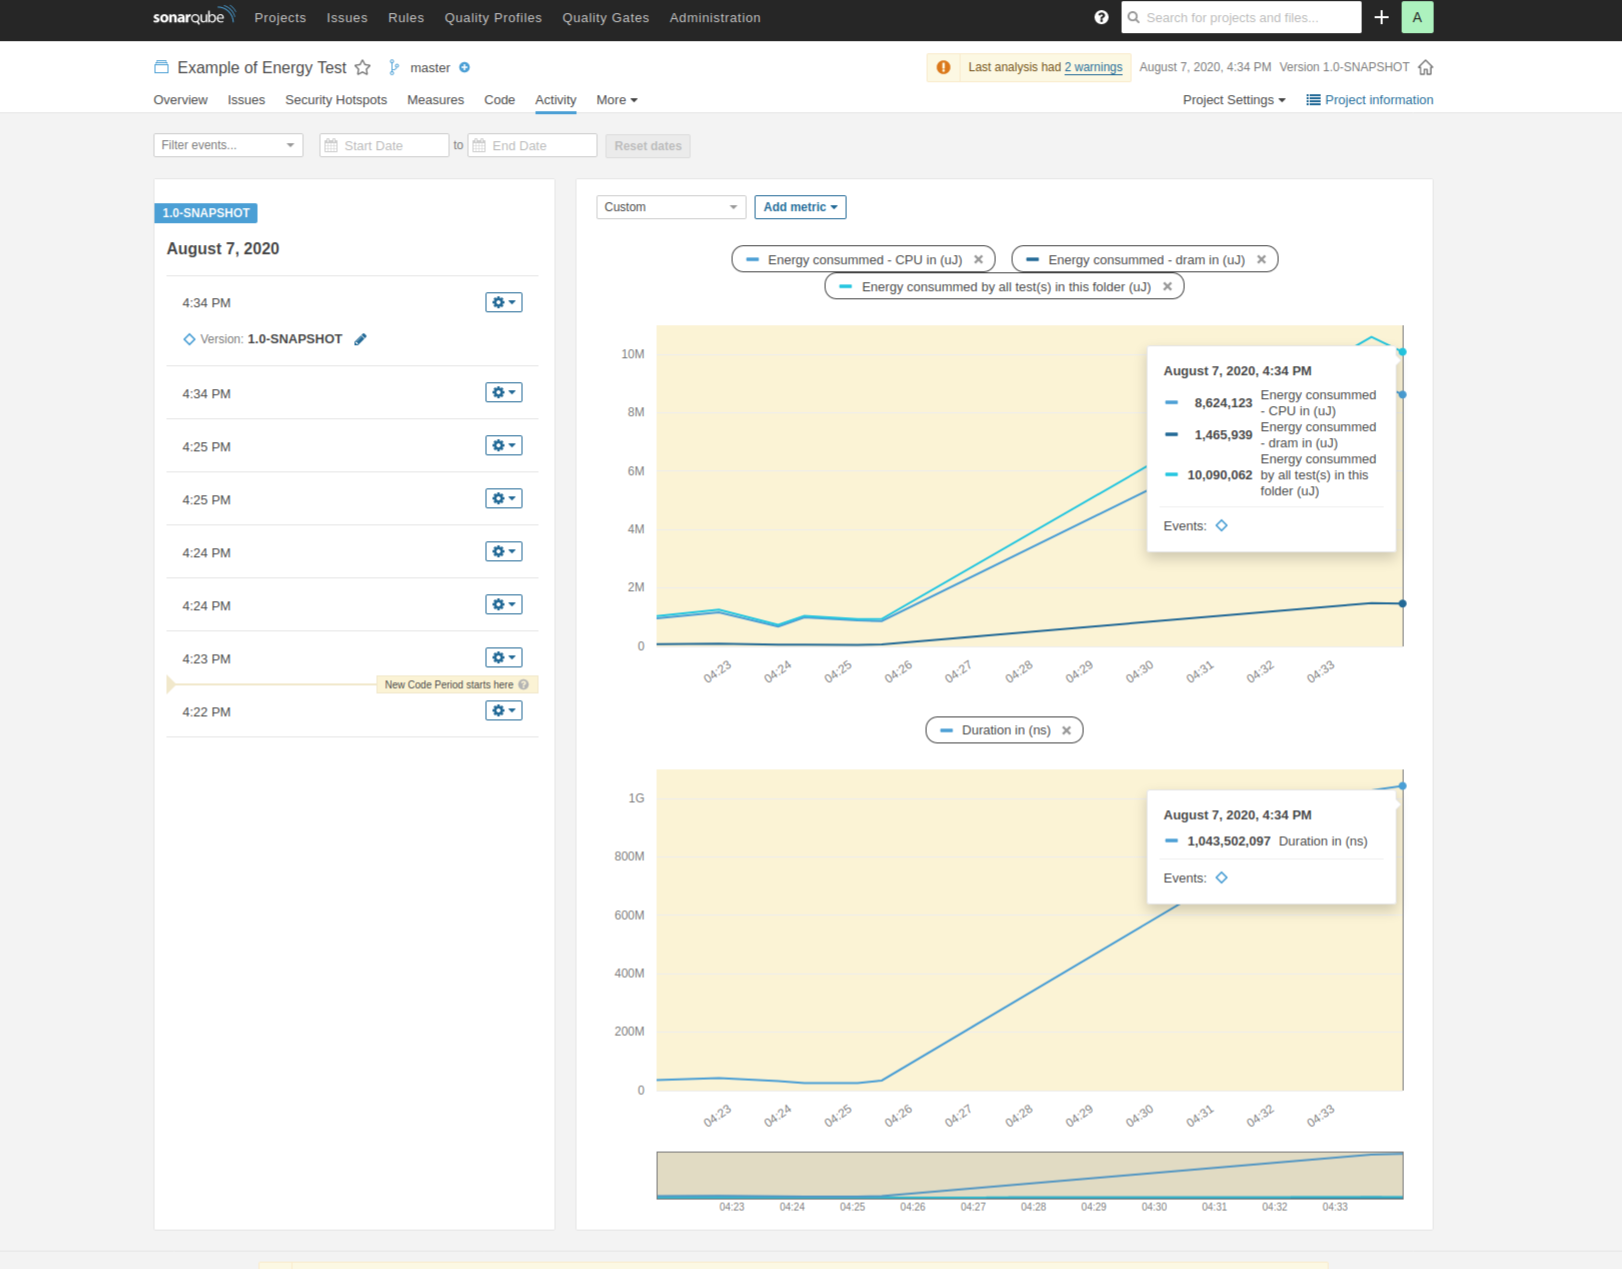
\includegraphics[width=.9\linewidth]{imgs/JunitSonarplugin}}
    \caption{Example of the Junit Sonar Plugin}\label{fig:sonar_plugin}
\end{figure}
